\documentclass[a4paper, 12pt, oneside]{scrbook}

\usepackage[backend=bibtex]{biblatex}
\usepackage[ngerman]{babel}		
\usepackage[T1]{fontenc}	  	
\usepackage[utf8]{inputenc}
\usepackage[hidelinks]{hyperref}
\usepackage{graphicx}
\usepackage{epstopdf}
\usepackage{float}
\usepackage{acronym}
\usepackage{booktabs}
\usepackage{caption}
\usepackage{csquotes}
\usepackage{fancyhdr}
\usepackage{url}
\usepackage{pdfpages}
\usepackage{mathtools}
\usepackage{float}
\usepackage{array}
\usepackage{tabularx}
\usepackage{etoolbox}

\renewcommand*{\headfont}{\normalfont}
\renewcommand*{\multicitedelim}{\addsemicolon\space}
\renewcommand*{\arraystretch}{1.5}
\renewcommand{\headsep}{15pt}

\setlength{\parskip}{1.5ex}

\renewcommand*\chapterpagestyle{fancy}

\pagestyle{fancy}
\renewcommand{\headrulewidth}{0.5pt}
\renewcommand{\footrulewidth}{0.5pt}

\fancyhead{} % clear all header fields
\fancyhead[L]{}
\fancyhead[C]{}
\fancyhead[R]{\nouppercase{\leftmark}}
\fancyfoot{} % clear all footer fields
\fancyfoot[L]{Viktor Rechel}
\fancyfoot[C]{}
\fancyfoot[R]{\thepage}

\newenvironment{conditions*}
{\par\vspace{\abovedisplayskip}\noindent
	\tabularx{\columnwidth}{>{}l<{} @{\ : } >{\raggedright\arraybackslash}X}}
{\endtabularx\par\vspace{\belowdisplayskip}}

\renewcommand{\title}{Lösung des Traveling-Salesman-Problem mithilfe einer parallelisierten Anwendung der Optimierung durch den Ameisen-Algorithmus}
\renewcommand{\author}{Viktor Rechel}
\newcommand{\doctype}{Studienarbeit}

\newcommand{\Matrikelnummer}{6335802}
\newcommand{\Kurskuerzel}{Inf15A}
\newcommand{\Company}{DHBW Mosbach}
\newcommand{\Gutachter}{Dr. Carsten Müller}

\addbibresource{bib/bibliography.bib}

\begin{document}
\pagestyle{fancy}

\frontmatter
\begin{titlepage}
\renewcommand{\headrulewidth}{0.0pt}
\pagestyle{empty}
\vspace{10mm}

\begin{center}
	\vspace{5mm}
	
	\huge \title
	
	\vspace{14.2pt}
	
	\large \doctype
	
	\vspace{42.6pt}
	
	\small des Studienganges Angewandte Informatik an der \\
	\large Dualen Hochschule Baden-Württemberg Mosbach
    
    \vspace{14.2pt}
	
	\begin{figure}[h!]
		\centering
		
\includegraphics[width=4cm]{images/logo.jpg}
	\end{figure}
	
	\small von \\
	\large \author
\end{center}

\vspace{98.6pt}

\begin{table}[h]
    \centering
    \begin{tabular}{ll}
        \small Bearbeitungszeitraum                 & 2 Semester; 6 Monate                     \\
        \small Matrikelnummer, Kurs                & \Matrikelnummer, \Kurskuerzel    \\
        \small Hochschule                     & \Company       \\
        \small Gutachter der Dualen Hochschule      & \Gutachter        \\
    \end{tabular}
\end{table}

\vspace{49.7pt}

\fancypagestyle{empty}{
  \fancyhf{}
  \fancyfoot[C]{\today}
}

\end{titlepage}
\addchap*{Abstract}

\fancyhead{} % clear all header fields
\fancyhead[L]{}
\fancyhead[C]{}
\fancyhead[R]{Abstract}
\fancyfoot{} % clear all footer fields
\fancyfoot[L]{Viktor Rechel}
\fancyfoot[C]{}
\fancyfoot[R]{\thepage}
\addchap*{Zusammenfassung}
\thispagestyle{fancy}
\renewcommand{\headrulewidth}{0.5pt}
\renewcommand{\footrulewidth}{0.5pt}

\fancyhead{} % clear all header fields
\fancyhead[L]{}
\fancyhead[C]{}
\fancyhead[R]{Zusammenfassung}
\fancyfoot{} % clear all footer fields
\fancyfoot[L]{Viktor Rechel}
\fancyfoot[C]{}
\fancyfoot[R]{\thepage}

\tableofcontents
\pagestyle{fancy}
\renewcommand{\headrulewidth}{0.5pt}
\renewcommand{\footrulewidth}{0.5pt}

\fancyhead{} % clear all header fields
\fancyhead[L]{}
\fancyhead[C]{}
\fancyhead[R]{\nouppercase{\leftmark}}
\fancyfoot{} % clear all footer fields
\fancyfoot[L]{Viktor Rechel}
\fancyfoot[C]{}
\fancyfoot[R]{\thepage}

\chapter*{Abkürzungsverzeichnis}
\thispagestyle{fancy}
\renewcommand{\headrulewidth}{0.5pt}
\renewcommand{\footrulewidth}{0.5pt}

\fancyhead{} % clear all header fields
\fancyhead[L]{}
\fancyhead[C]{}
\fancyhead[R]{Abkürzungsverzeichnis}
\fancyfoot{} % clear all footer fields
\fancyfoot[L]{Viktor Rechel}
\fancyfoot[C]{}
\fancyfoot[R]{\thepage}

\begin{acronym}
\end{acronym}
\addcontentsline{toc}{chapter}{Abkürzungsverzeichnis}

\cleardoublepage
\phantomsection
\addcontentsline{toc}{chapter}{Abbildungsverzeichnis}
\listoffigures
\pagestyle{fancy}
\renewcommand{\headrulewidth}{0.5pt}
\renewcommand{\footrulewidth}{0.5pt}

\fancyhead{} % clear all header fields
\fancyhead[L]{}
\fancyhead[C]{}
\fancyhead[R]{\nouppercase{\leftmark}}
\fancyfoot{} % clear all footer fields
\fancyfoot[L]{Viktor Rechel}
\fancyfoot[C]{}
\fancyfoot[R]{\thepage}

\cleardoublepage
\phantomsection
\addcontentsline{toc}{chapter}{Tabellenverzeichnis}
\listoftables
\pagestyle{fancy}
\renewcommand{\headrulewidth}{0.5pt}
\renewcommand{\footrulewidth}{0.5pt}

\fancyhead{} % clear all header fields
\fancyhead[L]{}
\fancyhead[C]{}
\fancyhead[R]{\nouppercase{\leftmark}}
\fancyfoot{} % clear all footer fields
\fancyfoot[L]{Viktor Rechel}
\fancyfoot[C]{}
\fancyfoot[R]{\thepage}

\mainmatter

\chapter{Einleitung}
\chapter{Stand der Technik \& Forschung}
\section{Traveling Salesman Problem}

\subsection{Beschreibung des Problems}

\subsection{Menge der Möglichkeiten in Bezug auf Anzahl der Städte}
\section{Ant Colony Optimization}{
	
}
\chapter{Konzeptionierung}
\pagestyle{fancy}
\renewcommand{\headrulewidth}{0.5pt}
\renewcommand{\footrulewidth}{0.5pt}

\fancyhead{} % clear all header fields
\fancyhead[L]{}
\fancyhead[C]{}
\fancyhead[R]{\nouppercase{\leftmark}}
\fancyfoot{} % clear all footer fields
\fancyfoot[L]{Viktor Rechel}
\fancyfoot[C]{}
\fancyfoot[R]{\thepage}

\section{Architektur}{
	Die Architektur wurde inhaltlich so aufgeteilt, dass eine modulare Implementierung möglich ist. So wurden die vier folgenden Bereiche definiert: Persistenz, Applikation, TSP und ACO
	
	Der Begriff der Persistenz beschreibt in diesem Fall zusätzlich zum dauerhaften Abspeichern der Daten, auch das Einlesen der verschiedenen Problemstellungen.
	\newline
	Applikation umfasst den Teil des Programms, der sich nicht direkt mit Daten befasst aber auch nicht zur Problemlösung beiträgt, wie die zwei folgenden Bereiche.
	\newline
	Innerhalb des Begriffs TSP werden alle nötigen Parameter und Methoden behandelt, die basierend auf dem Traveling Salesman Problem notwendig werden. 
	\newline
	Zuletzt gibt es in der Architektur noch das Feld ACO, welches die komplette Berechnung des zu lösenden Problems übernimmt. In dem Fall, dieser Arbeit handelt es sich um das TSP. Allerdings könnte das Problemfeld auch dadurch ausgewechselt werden, dass der Bereich TSP um das neue Problem ersetzt wird.
	
	\subsection{Persistenz}
	Um ein starres Definieren des Problems innerhalb der Applikation zu verhindern, werden zu Beginn des Programms alle Parameter, wie Städtematrix, Wahrscheinlichkeiten und Lösungsparameter aus einer gegebenen XML-Datei eingelesen. Durch eine Bearbeitung der XML ist ein einfaches Abändern der Problemstellung möglich. Hierdurch ist auch gesichert, dass die Algorithmen effizient getestet werden können, da mehrere verschiedenen bekannte Testwerte benannt werden können.
	
	\subsection{Applikation}
	Wie bereits genannt, liegt bei der vorliegenden Architektur ein Fokus auf Modularität, Portabilität und Usability. Aber auch auf verlässliche und effiziente Algorithmen muss geachtet werden. Daher wird für die Wahrscheinlichkeitsberechnung die externe Klasse MersenneTwisterFast \footnote{s. http://www.math.sci.hiroshima-u.ac.jp/~m-mat/MT/emt.html} genutzt, welche eine bessere Distribution der Pseudozufallszahlen bieten als die Default-Implementierung in Java.
	\footnote{Um eine einfache und schnelle Benutzung zu gewährleisten, wird in dieser Arbeit darauf verzichtet echte Zufallszahlen zu nutzen, die beispielsweise aus Weltallstrahlung berechnet werden. Diese seien hier nur zur Vollständigkeit halber erwähnt.}
	Ein weiterer Bestandteil des Applikationsbereichs werden das Logging der Arbeitsvorgänge, sowie die zentrale Konfiguration der Problemstellung auf der die Lösung basiert.
	
	\subsection{TSP}
	Der Bereich des TSP definiert sich in dieser Architektur rein durch die Städte-Objekte, welche zur Darstellung der Städtematrix genutzt werden. Der einzige andere Bestandteil ist die zentrale Aufstellung der Städtematrix, die von den restlichen Klassen nur kopiert wird.
	
	\subsection{ACO}
	Um den Ameisenalgorithmus umzusetzen sind deutlich mehr Aufwände nötig, als zur Darstellung des TSP. Hier werden mindestens eine Ameisenkolonie benötigt \footnote{Die Architektur würde bei ausreichenden Systemressourcen auch eine parallele Berechnung mehrerer Städtematrizen erlauben},
	sowie je Kolonie mehrere Ameisen.
	\newline
	Die Ameisen werden in der Applikation als einzelne Threads gestartet, die über eine CyclicBarrier kontrolliert werden. Dies erlaubt ein möglichst effizientes Parallelisieren der Lösung.
	
	\subsection{Arbeitsweise der Architektur}
	Die einzelnen Abschnitte der Architektur wurden bereits erklärt. Aber das Zusammenspiel der einzelnen Komponenten und der eigentliche Arbeitsablauf des Systems wurde noch nicht beschrieben. Im Folgenden wird ein Beispiel so durchgeführt, wie es auch die geplante Architektur umsetzen würden.
	\begin{figure}[h]
		\centering
		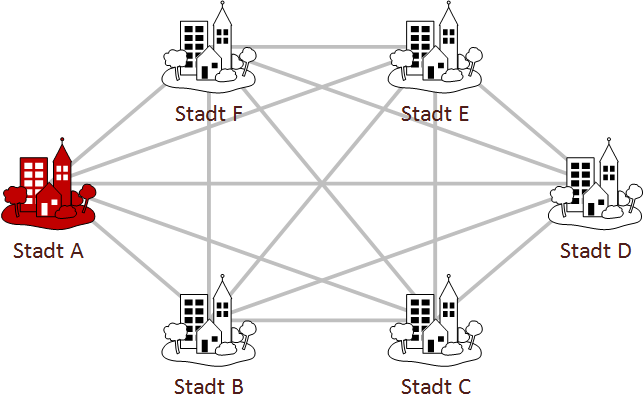
\includegraphics[width=0.9\linewidth]{images/TSP_ACO_numerisch.png}
		\caption{Darstellung des TSP-Beispiels zur Darlegung der Arbeitsweise der Architektur}
		\label{tspAcoNumerisch}
	\end{figure}
}
\section{UML-Diagramm}{

}
\section{Umsetzung der SOLID-Prinzipien}{
	Um eine saubere und übersichtliche Implementierung gibt es heutzutage eine Vielzahl von Regelwerken, Anleitungen und Vorgaben. Eine Sammlung von Grundsätzen sind die SOLID-Prinzipien. SOLID steht für \textbf{S}ingle Responsibility, \textbf{O}pen/Closed, \textbf{L}iskov Substitution, \textbf{I}nterface Segregation und \textbf{D}ependency Inversion.
	Alle diese Eigenschaften werden im Folgenden kurz erklärt und dann ihre Verwirklichung in der Architektur gezeigt.
	
	\subsection{Single Responsibility}
	Das Single-Responsibility-Prinip umschreibt den Zustand, dass Klassen max. eine Zuständig haben sollen. Klassen dürfen nicht mehrere Aufgabengebiete gleichzeitig übernehmen, da hierdurch eine Änderung an dieser Klasse zu einer Änderung mehrerer Komponenten führt und dadurch die ganze Struktur beeinflusst werden kann.
	Stattdessen wird die Software in mehrere kleinere Klassen aufgeteilt, die jeweils einen Teil übernehmen. Hierdurch ist zum Einen die Struktur einfacherer erkennbar und nachvollziehbar, da die Klassen eindeutiger definiert sind und der Code besser zusammengefasst ist. Zum Anderen sind die Abhängigkeiten aber auch auf ein Minimum reduziert.
	
	In der vorliegenden Konzeption ist dieser Grundsatz dadurch erfüllt, dass die Berechnungslogik an die Ameisen ausgegliedert ist, welche selbst keine Manipulation vornehmen. Die Ameisenkolonie hingegen funktioniert nur als Quelle der Threads und behält einige wenige Kolonie-spezifische Attribute bereit, sonst nichts.
	Andere Anwendungen, wie das Logging, das Einlesen von Konfigurationsdateien und die Zufallszahlerzeugung wurde alle in getrennte Klassen ausgegliedert, die zentral in \textit{Configuration} initialisiert werden.
	
	\subsection{Open / Closed}
	Die Open-Closed-Eigenschaft, welche eine moderne Software besitzen muss, umschreibt den Umstand, dass ein möglichst modularer Aufbau genutzt wird. So sollen Klassen so aufgebaut sein, dass bei einer Erweiterung keine Änderung bestehenden Codes notwendig wird, sondern zum Beispiel über das Implementieren eines Interfaces die alten Strukturen genutzt werden können.
	Unterscheiden muss man hier zwischen einer Erweiterung und einer Änderung. Die Software muss nicht und soll auch nicht auf eine einfache Änderung ausgelegt sein. Der Code, welcher erfolgreich implementiert wurde, soll auch in seinem Funktionsumfang weiter genutzt werden. Die bestehenden Implementierungen müssen keine Schnittstellen zur einfach Änderung enthalten.
	
	Durch die Schlichtheit der entworfenen Architektur und den auf die Problemstellung zugeschnittenen Charakter ist eine Umsetzung des Open-Closed-Prinzips nur in geringem Umfang möglich. Alleine die Parser können hiernach umgesetzt werden, in dem ein Interface eingesetzt wird. Dadurch wird ermöglicht in Zukunft auch andere Datei-Typen akzeptieren zu können.
	In der restlichen Implementierung ist eine Umsetzung nicht hilfreich oder zweckdienlich.
	
	\subsection{Liskov Substitution}
	Die Substitutionsregel von Liskov besagt, dass es möglich sein sollte eine Klasse in einem beliebigen Aufruf auch durch eine Subklasse aus zu tauschen ohne den Programmablauf zu ändern.
	Folglich müssen entweder die Implementierung abgestimmt sein, dass ein Austauschen generell möglich ist. Dies ist aber meist nicht zweckdienlich.
	Andererseits ist es auch möglich, über eine abstrakte Klasse zu arbeiten, die für Methodenaufrufe benutzt wird. So wird der Programmablauf nicht durch unterschiedliche Klassentypen unterbrochen, sondern der Entwickler ist in der Pflicht die abstrakte Klasse entsprechend umzusetzen.
	
	Ähnlich zu der Open-Closed-Eigenschaft ist auch diese Leitlinie in dem vorliegenden Entwurf nur sehr schwierig umzusetzen. Da von einem Hineinquetschen von Regeln und Leitlinien in eine Architektur generell abzuraten ist, wurde auf eine Umsetzung der Substitutionsregel generell verzichtet.
	
	\subsection{Interface Segregation}
	Die Trennung der Interfaces zielt darauf ab, Klassen nicht dazu zu zwingen Methoden zu implementieren, die gar nicht benötigt werden. So müssen in den meisten Programmiersprachen alle Methoden eines Interfaces zwingend umgesetzt werden. Dies führt aber meist zu einer aufgeblähten Codestruktur, da unnötige Methoden implementiert werden müssen, aber nie benutzt werden.
	Indem man die Interfaces in kleine Interfaces unterteilt ist es möglich durch eine Implementierung von mehrerer Interfaces auf das gleiche Ergebnis zu kommen ohne den Zwang alle anderen Interface auch umzusetzen.
	
	Aufgrund des Mangels an Interfaces in der Codestruktur der hier behandelten Architektur ist auch diese Regel nicht umgesetzt. Sobald Interface allerdings zum Einsatz kommen, muss diese Regel umgesetzt werden.
	
	\subsection{Dependency Inversion}
	Die Abhängigkeitsumkehr-Regel besagt, dass Module auf höheren Ebenen nicht auf Module niederer Ebenen angewiesen sein dürfen. Ähnlich zu den anderen Richtlinien sollen auch hier abstrakte Klassen und Interface zur Abstraktion genutzt werden.
	Allerdings gibt es noch den Zusatz, dass Abstraktionen niemals von einer detaillierten Implementierung abhängen dürfen.

	Wie bei den anderen Interface-Umsetzungen ist auch hier eine Umsetzung nicht hilfreich bzw. möglich. Dennoch sei auch hier erwähnt, dass eine Benutzung der Regel zu einfacher zu wartenden Code führt.
}
\section{Ausgewählte Algorithmen}{
\label{algorithms}
	Bereits vorgestellt wurden die einzelnen Bestandteile der Architektur, sowie die Architektur als Gesamtbild gezeigt. Im Folgenden sollen beispielhaft die verwendeten Algorithmen thematisch vorgestellt werden. So werden die zentralen Methoden zur Berechnung der Iterationen aus Sicht der Ameisen vorgestellt, sowie auch das Verhalten der Pheromonänderung. Zusätzlich wird die Methode zum Töten einer Ameise beschrieben, welche in so gut wie keiner Implementierung zu finden ist.
	
	\subsection{Ant - iteration()}
	In dem \ref{parameter} wurde bereits die Berechnung beschrieben, die für jede neue Streckenauswahl von den Ameisen durchgeführt werden muss. Diese Berechnung wird in der Implementierung in der Iteration der Ameisen umgesetzt. Pro Durchgang bzw. Iteration wird also jede besuchbare, angrenzende Stadt betrachtet und auf Ihre Attraktivität untersucht. Überwiegt der Pheromonwert $\tau$, welcher über Alpha gewichtet ist, über dem heuristischen Faktor $\eta$, der mit Beta verrechnet wird, so wird die bisher von der Kolonie gewählten Strecke gewählt. Diese Berechnung wird für alle Städte berechnet und dann verglichen. Die im Vergleich attraktivste Strecke wird in diesem Zusammenhang dann gewählt.
	Nachdem eine Strecke gewählt wird, verteilt die Ameise auf der Strecke ihre Pheromone indem der Kolonie ein Pheromonwert mitgeteilt wird, welcher auf den bisherigen addiert werden muss.
	
	\subsection{Colony - killAnt()}
	Ebenfalls in dem in Abbildung \ref{uml_class} gezeigten UML-Diagramm erkennbar ist, dass die Ameisenkolonie die Möglichkeit besitzt einzelne Ameisen zu "töten". 
	Diese Methode sollte in einem einwandfreiem Programm keinerlei Verwendung finden, allerdings kann man sich nicht auf eine dauerhafte fehlerfreie Implementierung verlassen. Im Bereich der Software Tests ist dies durch das Prinzip "Fehlen von Fehlern" beschrieben. Dieses sagt aus, dass erfolgreiche Tests nur bestätigen, dass keine Fehler gefunden wurden. Es kann nicht ausgesagt werden, dass keine Fehler vorliegen.\footnote{vgl. \cite{bibid}}
	
	Denn die Methode hat die Funktion, im Falle des Fehlverhaltens eine Ameise aus der Liste der aktiven Ameisen bzw. Threads zu löschen und den Thread zu stoppen.
	Genutzt werden wird diese vor allem im Bereich der aufgefangenen Fehler innerhalb der Implementierung der Ameisen. Sollte eine aufgetretene Exception schwerwiegend und unlösbar sein, wird die Applikation automatisch die Funktion aufrufen.
	
	\subsection{Colony - updatePheromone()}
	Schon mehrfach erwähnt wurden die Pheromonwerte, die Pheromonmatrix, sowie die Pheromonverteilung. All diese Begriffe sind auf die Ameisenkolonie zurückzuführen. Denn diese enthält die Pheromonmatrix, die von den Ameisen zur Berechnung der Iteration benutzt wird. Um diese aktuell zu halten wird diese von jeder Ameise nach jeder Iteration upgedatet. 
	
	Dabei wird die Funktion \textit{updatePheromone} der Kolonie aufgerufen und ein neuer Wert übergeben. Die Kolonie schreibt diesen dann in die zentrale Matrix, sodass der neue Wert bei der nächsten Iteration allen Ameisen ersichtlich ist. Durch diesen gleichzeitig und unübersichtlichen Zugriff auf die Matrix, muss diese Funktion synchronisiert ablaufen um einen Datenverlust zu verhindern.
	
}
\section{Parameteranalyse}{

}
\section{Sensitivitätsanalyse}{

}
\chapter{Implementierung}
\section{Klassendiagramm}
\section{Beschreibung der Implementierung}
Um die Funktionsweise der Softwarelösung zu verstehen, ist eine klare Übersicht über die einzelnen Bestandteile notwendig. Diese wird im Folgenden über ein Klassendiagramm inkl. Beschreibung gegeben. Danach werden noch die einzelnen Abschnitte in ihrer Funktion beschrieben.

\subsection{Klassendiagramm}
Bevor auf den genauen Funktionsablauf der Applikation eingegangen wird, sollte zuerst ein Überblick auf die Implementierung gegeben werden. Hierzu ist in Abbildung \ref{classDiagram} der komplette Umfang aller Klassen aufgezeigt
\footnote{Aus Gründen der Übersichtlichkeit wurden die getter- und setter-Methoden weggelassen, um die Abbildung nicht über zu dimensionieren}. Leicht erkennbar ist, dass der größte Teil der Logik innerhalb des aco-Pakets - welches unter anderem Ant und Colony enthält - stattfindet. Landscape, also die Klasse welche das \ac{TSP} beschreibt, dient nur als Schnittstelle zur Abfrage der Distanzen zwischen den Städten.

\begin{figure}[h]
	\centering
	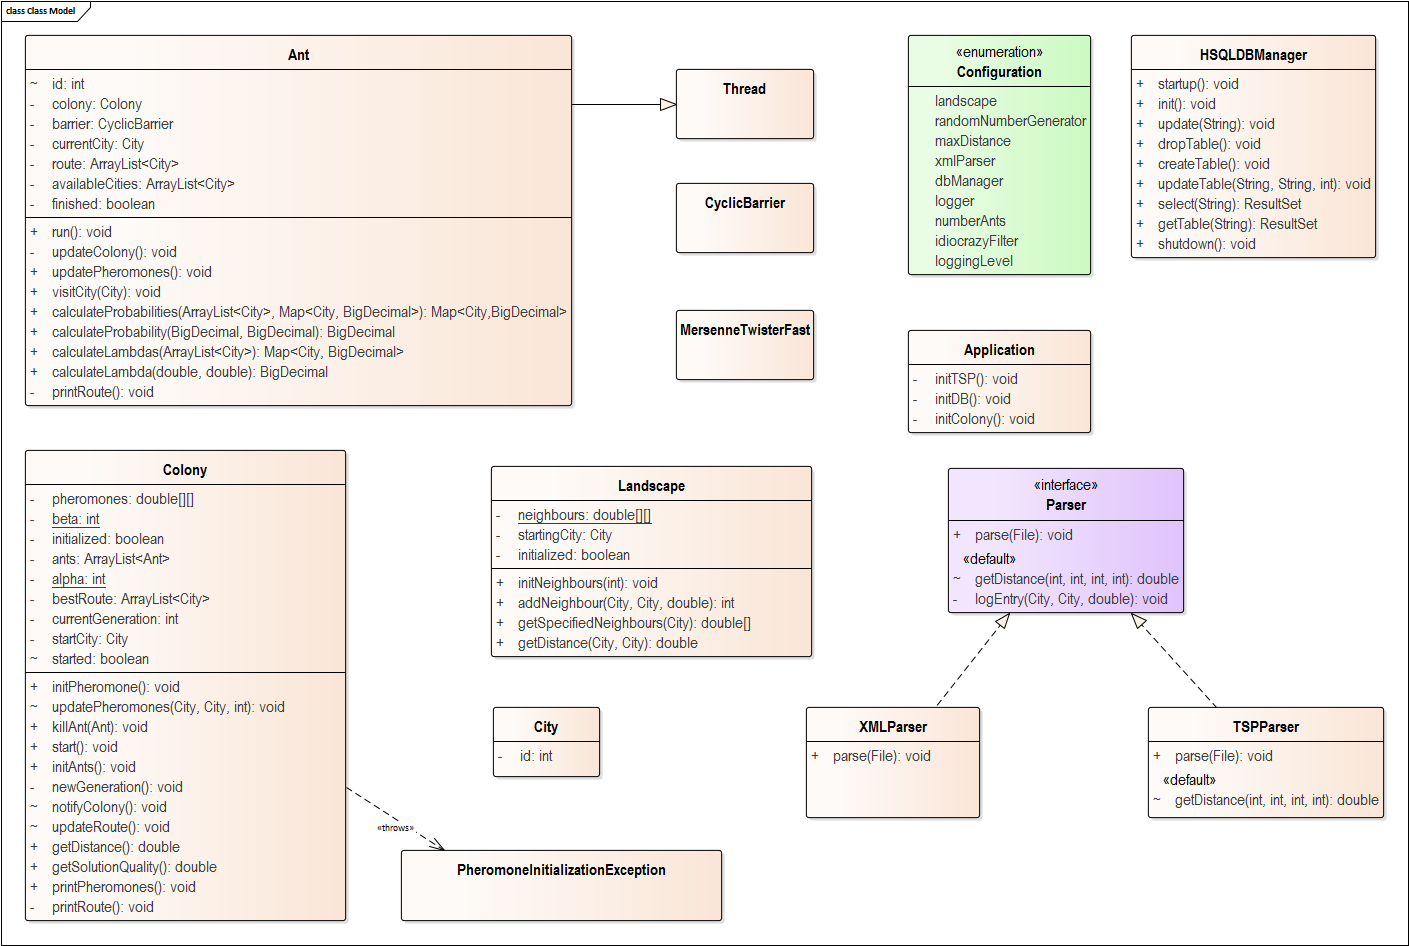
\includegraphics[width=\linewidth]{../../../01_uml/classModel.png}
	\caption{Klassendiagramm der vorliegenden Softwarelösung}
	\label{classDiagram}
\end{figure}

\subsection{Persistenz}
Um die Ergebnisse der einzelnen Generationen persistent abspeichern zu können, ohne den Speicherverbrauch des Programms ansteigen zu lassen, wird eine Datenbank-Anbindung an eine HSQLDB-Datenbank verwendet. Um die Performance möglichst hoch und den Datenbankumfang möglichst klein zu halten, werden in dieser allerdings nur zwei Tabellen erstellt und verwaltet.

Zum Einen wird von jeder Generation, welche den Algorithmus durchlaufen hat, die beste Route erfasst und abgespeichert. Hierbei besteht ein Tabelleneintrag lediglich aus einer Zufalls-ID, der Route als String und der Distanz als Double. 

Zum Anderen wird eine Tabelle zur Verfolgung der Verbesserung angelegt. In der Historie wird eine Route nur dann abgespeichert, wenn diese sich im Vergleich zur vorherigen auch verbessert hat. Somit besteht diese aus den gleichen Attributen, wie die Generationen-Tabelle, mit dem Zusatz, dass auch die Generation, welche die Verbesserung verursacht hat, mit einer Ganzzahl abgespeichert wird.

\subsection{Applikation}
Dem Bereich der Applikation sind im Grund zwei Klassen zu zu ordnen: die Applikation selbst, sowie die Konfiguration. Hierbei ist die Konfiguration für alle Klassen und Instanzen innerhalb des Programms erreichbar und enthält alle Konfigurationen, sodass diese zentral angepasst werden können. 

Auch wird über die Konfiguration der Logger angesprochen, sodass hierzu keine eigene Klasse notwendig wird. Die Applikation hat als einzigen Zweck die Problemstellung einlesen zu lassen, sowie die Architektur zu initialisieren, um diese dann zu starten. Nachdem die Kolonie gestartet ist, wartet die Applikation nur noch darauf, die Datenbank wieder schließen zu dürfen.

\subsection{TSP}
Der \ac{TSP}-Bereich der Architektur dient zu aller erst der Verdeutlichung des Aufbaus. So soll durch die Verwendung der City-Klasse statt einfachen Integern das Verständnis gefördert werden. Innerhalb der Landscape-Instanz - welche in der Konfiguration zentral initialisiert wird -  wird die zweidimensionale Matrix der Distanzen zwischen den Städten bereit gehalten. 

Über diese Matrix kann immer zentralisiert der Wert von den Ameisen nachgefragt werden, ohne eine unnötige Berechnung durchzuführen. Ebenso fördert dieser Aufbau die Sicherung der Funktionsfähigkeit, da einfacher sichergestellt werden kann, dass die Distanzen richtig berechnet werden. Ein weiterer Vorteil ist, dass die Ameisen hier eine Liste von Nachbarn der derzeitigen Position nachfragen können, indem sie ihren derzeitigen Standort übergeben. Dies vereinfacht das Konzept bei der Berechnung innerhalb der Ameisen-Klasse.

\subsection{ACO}
Der hauptsächliche Teil der Berechnung wird innerhalb des \ac{ACO}-Bereichs durchgeführt. Denn hier befindet sich die Ameisenkolonie, als Verwaltungsorgan, und die Ameisen, welche als Threads gleichzeitig auf die Suche nach der bestmöglichen Lösung gehen.

Von der Kolonie werden die Ameisen insofern verwaltet, dass die Threads über diese Klasse gestartet werden, sowie hier auch die Ergebnisse abgeliefert werden. Nach jeder Generation wird innerhalb der Kolonie für jede Ameise eine Auswertung gestartet, ob die Route besser war als die derzeit beste. Sollte dies der Fall sein, wird die alte Route mit der neuen Route überschrieben.

Unabhängig davon ob eine neue beste Route gefunden wurd oder nicht, wird nach jeder Generation von Ameisen ein Update auf die Pheromonmatrix durchgeführt. Hierbei meldet jede Ameise für jeden Weg, den sie zwischen zwei Städten gegangen ist, einen Wert, welcher auf den derzeitigen Pheromonwert addiert werden soll. Hierfür iteriert eine Ameise über die Route, welche sie sich gemerkt hat, und ruft die updatePheromone-Methode der Kolonie auf, mit dem Wert $1/distance$, wobei $distance$ der Distanz zwischen der Stadt, über welche gerade iteriert wird, und der Folgestadt beträgt. 

Die restliche Berechnungsarbeit wird von den einzelnen Ameisen bzw. Threads bewältigt. Diese berechnen ab dem Startpunkt für alle möglichen Nachbarn
\footnote{Ein Nachbar ist dann erreichbar, wenn dieser noch nicht in der Route vorgekommen ist, also noch nicht besucht wurde.} einen $\lambda$-Wert\footnote{Beschrieben wurde diese Berechnung bereits in Kapitel \ref{parameter}}. 
Als nächstes werden alle $\lambda$s aufsummiert, um mit den einzelnen $\lambda$s der Städte dividiert durch die Summe die Wahrscheinlichkeit zu berechnen. Hierdurch wird beschrieben, dass Städtepaare, welche eine kurze Distanz besitzen, sowie einen hohen Pheromonwert besitzen, deutlich wahrscheinlicher besucht werden. Hierbei kann eine unterschiedliche Gewichtung vorgenommen werden, wie in Kapitel \ref{parameter} und Kapitel \ref{analyse} beschrieben wurde.

Nachdem für alle erreichbaren Städte die Wahrscheinlichkeiten berechnet wurden, wird eine Zufallszahl bestimmt. Sollte eine Wahrscheinlichkeit für eine Stadt höher sein, als die Zufallszahl so wird die Berechnung an dieser Stelle beendet und die Ameise besucht diese Stadt. Sollte diese Bedingung für keine einzelne Stadt erfüllt werden, so werden die Wahrscheinlichkeiten solange aufsummiert bis die Summe größer ist als die Zufallszahl. Die Stadt, bei welcher diese Schwelle überschritten wird, wird dann von der Ameise aufgesucht.

Sobald jede Ameise ihre Route beendet hat und wieder bei der Anfangsstadt angekommen ist, wird über die CyclicBarrier zentral eine Methode innerhalb der Kolonie angestoßen. Diese fordert nach und nach jede Ameise auf, das Ergebnis zu melden, um die Pheromonmatrix zu aktualisieren. Nachdem die Kolonie vollständig aktualisiert wurde, ist die derzeitige Generation beendet und es wird eine neue generiert und gestartet.
\section{ER-Diagramm}{
	
}
\section{Komponenten-Diagramm}{
	
}
\section{Paket-Diagramm}{
	
}
\section{Performance-Analyse}
Selbstverständlich ist für eine richtige Implementierung nicht nur wichtig, dass diese funktioniert. Sie muss dies auch möglichst performant und effizient tun. Hierzu werden mehrere Testläufe in Hinblick auf die Performance durchgeführt. Im Folgenden werden diese Testfälle beschrieben, sowie auch die Hardware, auf welcher die Tests durchgeführt werden. Ohne die Referenz zur verwendeten Hardware wäre eine Aussage über die Performance nur sehr bedingt verwendbar. In Abbildung \ref{hardware} sind die relevanten Komponenten aufgelistet. Zu beachten ist hierbei, dass AMD-Prozessoren allgemein eine höhere Multithreading-Performance besitzen, welche in der vorliegenden Software genutzt wird.
\begin{table}[H]
	\centering
	\setstretch{0.75}
	\begin{tabular}{c c c c c c c}
		Komponente & Name & Technische Daten\\
		CPU & AMD FX8350 & 8 Kerne, 4.2 GHz\\ 
		RAM & Kingston 99U5471 & 24 GB DDR3, 666 MHz  \\ 
	\end{tabular}
	\caption{Für Performance-Benchmarks verwendete relevante Hardware}
	\label{hardware}
\end{table}
Als Grundlage der Benchmarks wird das a280-\ac{TSP} verwendet um zum Einen eine standardisierte Grundlage zu erhalten und zum Anderen um eine genügend große Problemstellung zu erzeugen, die bezogen auf den Rechenaufwand auch relevant ist. Es wurden 8 parallele Threads gestartet, um eine hohe Auslastung der Hardware zu gewährleisten, ohne durch zu umfangreiches Threadhandling Performance einzubüßen. Die Applikation wurde genau 60 Sekunden lang betrieben, um einen einfachen Vergleichswert zu erhalten.

\newpage
\subsection{CPU-Auslastung}
Wie in Abbildung \ref{cpuUsage} zu sehen ist, beansprucht die Applikation durchgehend zwischen 60 und 70 Prozent. Dass keine 100 Prozent genutzt werden können, liegt daran, dass die Test-Umgebung nicht optimal ist. So wurden die Benchmarks auf einem Desktop-PC in normalen Betrieb mit gleichzeitiger Heim-Nutzung durchgeführt. Da für das Betriebssystem keine Priorisierung der Applikation vorliegt, wird diese mit anderen Programmen gleichgestellt und die Ressourcen auch dementsprechend verteilt.

\begin{figure}[h]
	\centering
	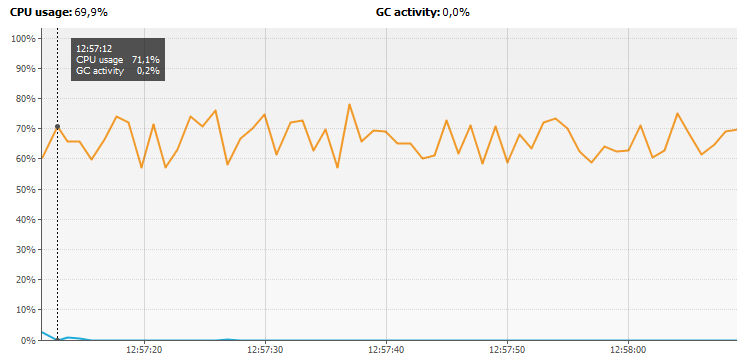
\includegraphics[width=0.9\linewidth]{images/cpuUsage.png}
	\caption{Aufzeichnung der CPU-Beanspruchung der Applikation über die gesamte Laufzeit}
	\label{cpuUsage}
\end{figure}

Würde die Applikation auf einer einwandfreien Test-Umgebung betrieben werden, würden bis zu 100 Prozent der CPU genutzt werden, was zu einer Verbesserung der Performance führen würde. Aber eine hohe Nutzung der CPU alleine kann nicht beschreiben, wie effizient ein Programm arbeitet. Hierzu sind noch andere Parameter notwendig, wie zum Beispiel die Nutzung des Hauptspeichers.

\subsection{Heap-Nutzung}
In Abbildung \ref{heapUsage} ist eine Statistik des benötigten Heaps der Applikation über die Laufzeit zu sehen. In blau markiert ist der benötigte Speicher im Heap zu einem bestimmten Zeitpunkt. In orange hinterlegt ist die Menge an Speicher, welche vom Programm allokiert wurde. Es lassen sich hierbei mehrere Aussagen ableiten. 

Zum Einen ist die Speicherallokierung konstant. Es werden vom Programm immer 2,4 GB an RAM belegt. Zum Anderen ist der Unterschied zwischen belegtem und allokierten Speicher teilweise enorm, was aber nicht auf die Arbeitsweise des Programms zurückzuführen ist. Zusätzlich lässt sich über die Grafik auch noch bestätigen, dass der GarbageCollector von Java zuverlässig nicht mehr benötigte Strukturen im Heap wieder frei gibt, was durch die lokalen Tiefpunkte im Heap-Verbrauch ersichtlich wird.

\begin{figure}[h]
	\centering
	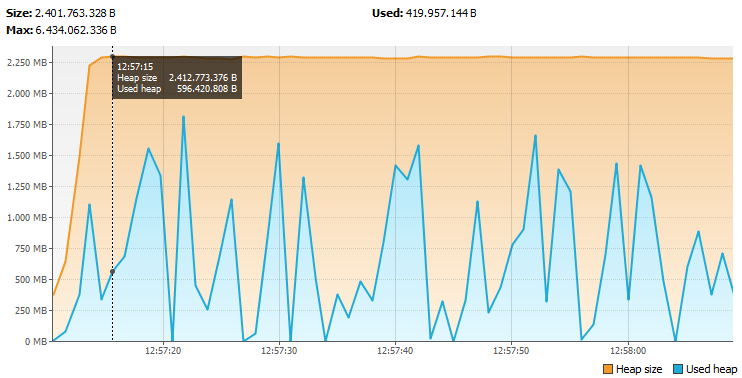
\includegraphics[width=0.9\linewidth]{images/heapUsage.png}
	\caption{Aufzeichnung des Speicherverbrauchs der Applikation über die gesamte Laufzeit. Blau markiert ist der derzeit verwendete Speicher, in orange der allokierte Speicher.}
	\label{heapUsage}
\end{figure}

Als möglichen Optimierungspunkt lässt sich hier der überdimensionierte Heap nennen. Mit 2,4 GB ist der Verbrauch zwar nicht so hoch, dass er eine Verwendung auf einer heutigen Hardware verhindert. Allerdings ist bei einem Anspruch einer möglichst effizienten Software dieser unnötige Verbrauch nicht haltbar.

\subsection{Anzahl Threads pro Minute}
Schlussendlich ist nicht die Auslastung der Hardware ausschlaggebend für die Performance eines Algorithmus, sondern wie effizient dieser rechnet. Als Richtwert kann in diesem Beispiel die Anzahl an Threads pro Minute herangezogen werden, da ein Thread einem Rechenschritt entspricht bzw. über die Anzahl an Threads auch die Anzahl an Generationen errechnet werden können. Die Anzahl an Generationen ist hierbei ein direkter Richtwert wie viele Routen abgelaufen werden konnten.

In Abbildung \ref{threadUsage} ist eine Statistik der in der Applikation aktiven Threads aufgezeigt. In blau werden die Daemon-Threads - hauptsächlich Systemthreads, wie beispielsweise der GarbageCollector - und in rot die Live-Threads gezeigt. Die Menge an aktiven Live-Threads beläuft sich im Durchschnitt auf 19. Für die Berechnung werden pro Generation acht Threads gestartet, welche nach der Generation auch wieder abgebaut werden. Somit ist auch hier wieder ein Overhead vom System vorhanden - in Summe 11 Live-Threads und 10 Daemon-Threads.

\begin{figure}[h]
	\centering
	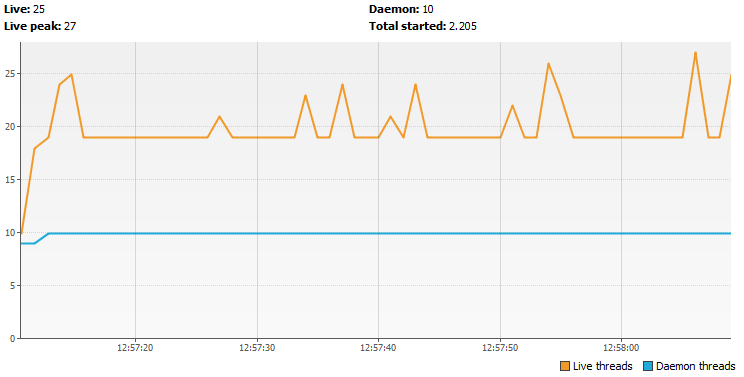
\includegraphics[width=0.9\linewidth]{images/threadUsage.png}
	\caption{Aufzeichnung der Menge an gleichzeitig aktiven Threads des Programms. In blau gezeichnet ist die Menge an Daemon-Threads, in orange die Anzahl an aktiven Live-Threads.}
	\label{threadUsage}
\end{figure}

Mithilfe der Datenerfassung lässt sich auch die genaue Anzahl an gestarteten Threads innerhalb der Applikation ermitteln. Innerhalb von 60 Sekunden wurden 2170 Threads bzw. Ameisen gestartet. Somit wurden ca 36,1 Ameisen pro Sekunde generiert. Teilt man diese Menge durch die Anzahl an Ameisen pro Generation (also acht) erhält man die Menge an Generationen pro Sekunde - in diesem Fall ca. 4,5.

\newpage
\subsection{Fazit zur Performance}
Nun wurden im Detail die relevanten Daten zur Performance genannt und analysiert. Als Fazit können einige Punkte genannt werden:
\begin{itemize}
	\item Die CPU wird fast vollständig genutzt
	\item Der Heap-Verbrauch ist akzeptabel, aber nicht optimal
	\item Es werden bei acht gleichzeitigen Ameisen 4,5 Generationen des a280-Problem pro Sekunde berechnet
\end{itemize}
Diese Aussagen ergeben eine relativ gute Bewertung der Applikation in Hinblick auf die Performance. Allerdings wurden bereits Schwachstellen erkannt. So ist die Belegung des Speichers im Vergleich zum wirklichen Verbrauch teilweise sehr hoch. Auch entsteht durch System-Threads ein recht großer Overhead. Im weiteren Entwicklungsverlauf dieser Applikation sollte in diesen Punkten noch eine Optimierung vorgenommen werden.
\chapter{Fazit}
\pagestyle{fancy}
\renewcommand{\headrulewidth}{0.5pt}
\renewcommand{\footrulewidth}{0.5pt}

\fancyhead{} % clear all header fields
\fancyhead[L]{}
\fancyhead[C]{}
\fancyhead[R]{\nouppercase{\leftmark}}
\fancyfoot{} % clear all footer fields
\fancyfoot[L]{Viktor Rechel}
\fancyfoot[C]{}
\fancyfoot[R]{\thepage}

Ich bin ein Fazit

\nocite{*}

\backmatter

\sloppy

\cleardoublepage
\phantomsection
\addcontentsline{toc}{chapter}{Literaturverzeichnis}
\printbibliography[title=Literaturverzeichnis]

\end{document}